\begin{figure}

   \setlength{\unitlength}{\textwidth}

   \begin{picture}(1,0.399)(0.01,0.77)
     % % % 90
     \put(0.03,1){\includegraphics[width=0.35\unitlength]{../FnP/gnuplot/vel_time_history_75.eps}}   
     \put(0.36,1){\includegraphics[width=0.35\unitlength]{../FnP/gnuplot/vel_time_history_175.eps}}
     \put(0.68,1){\includegraphics[width=0.35\unitlength]{../FnP/gnuplot/vel_time_history_375.eps}}
         
     \put(0.03,0.82){\includegraphics[width=0.35\unitlength]{../FnP/gnuplot/dis_time_history_75.eps}}   
     \put(0.36,0.82){\includegraphics[width=0.35\unitlength]{../FnP/gnuplot/dis_time_history_175.eps}}
     \put(0.68,0.82){\includegraphics[width=0.35\unitlength]{../FnP/gnuplot/dis_time_history_375.eps}}
     
 
     
     \put(0.55,0.79){$\displaystyle{\frac{tU}{D}}$}
     \put(0.2,0.79){$\displaystyle{\frac{tU}{D}}$}
     \put(0.85,0.79){$\displaystyle{\frac{tU}{D}}$}
     
      \put(0.02,1.07){$\displaystyle\frac{V}{D}$}
     \put(0.02,0.9){$\displaystyle\frac{A}{D}$}
 
     
     \put(0.08,0.9997){(a)}    
     \put(0.4,0.9997){(b)}    
     \put(0.72,0.9997){(c)}
     \put(0.08,0.8){(d)}    
     \put(0.4,0.8){(e)}    
     \put(0.72,0.8){(f)}
     
    
   \end{picture}

  \caption{ Time histories of displacement and velocity at \reynoldsnumber=22300, \ustar=175 and $\frac{c}{\rho\mathcal{A}U}=9.3\times10^{-1}$. The velocity time histories are presented for: (a) $m^*=1164$; (b) $m^*=10$; (c) $m^*=5$. The time history of displacement are presented for: (a) $m^*=1164$; (b) $m^*=10$; (c) $m^*=5$   As the mass ratio decreases the signal tend to transform from a sinusoidal towards a square signal and the displacement signal tend to move towards a triangular signal due to reduction in inertia.}
  
  \label{time_hostory_mstar_mass}
\end{figure}




